\subsection{Our Planetary System}
What does the solar system look like?
\begin{itemize}
\item There are eight major planets with nearly circular orbits.
\item Dwarf planets are smaller than the major planets and some have quite elliptical orbits.
\item Planets all orbit in same direction and nearly in same plane.
\end{itemize}
Comparative Planetology (find patterns among planets)
\begin{itemize}
\item Planets are very tiny compared to distances between them.
\item All large bodies in the solar system orbit in the same direction and in nearly the same plane and most rotate in the same direction
\item two planet types
\begin{itemize}
\item terrestrial
\item jovian
\end{itemize}
\item Many rocky asteroids and icy comets populate the solar system.
\end{itemize}
Exceptions:
\begin{itemize}
\item Uranus spins sideways
\item earth has a large moon
\item venus rotates backwards
\end{itemize}
Objects:
\begin{itemize}
\item sun
\begin{itemize}
\item Over 99.9\% of solar system's mass
\item Made mostly of H/He gas (plasma)
\item Converts 4 million tons of mass into energy each second
\end{itemize}
\item mercury
\begin{itemize}
\item Made of metal and rock; large iron core
\item Desolate, cratered; long, tall, steep cliffs
\item Very hot, very cold: 425C (day), –170C (night)
\end{itemize}
\item venus
\begin{itemize}
\item Nearly identical in size to Earth; surface hidden by clouds
\item Hellish conditions due to an extreme greenhouse effect
\item Even hotter than Mercury: 470C, day and night
\end{itemize}
\item earth
\begin{itemize}
\item An oasis of life
\item The only surface liquid water in the solar system
\item A surprisingly large moon
\end{itemize}
\item mars
\begin{itemize}
\item Looks almost Earth-like, but don't go without a spacesuit!
\item Giant volcanoes, a huge canyon, polar caps, more
\item Water flowed in distant past; could there have been life?
\end{itemize}
\item jupiter
\begin{itemize}
\item Much farther from Sun than inner planets
\item Mostly H/He; no solid surface
\item 300 times more massive than Earth
\item Many moons, rings
\begin{itemize}
\item Io (shown here): active volcanoes all over
\item Europa: possible subsurface ocean
\item Ganymede: largest moon in solar system
\item Callisto: a large, cratered "ice ball
\end{itemize}
\end{itemize}
\item saturn
\begin{itemize}
\item Giant and gaseous like Jupiter
\item Spectacular rings:Rings are NOT solid; they are made of countless small chunks of ice and rock, each orbiting like a tiny moon.
\item Many moons, including cloudy Titan
\end{itemize}
\item uranus
\begin{itemize}
\item Smaller than Jupiter/Saturn; much larger than Earth
\item Made of H/He gas and hydrogen compounds(H2O, NH3, CH4)
\item Extreme axis tilt
\item Moons and rings
\end{itemize}
\item neptune
\begin{itemize}
\item Similar to Uranus (except for axis tilt)
\item Many moons (including Triton)
\end{itemize}
\item dwarf planets
\begin{itemize}
\item Much smaller than major planets
\item Icy, comet-like composition
\item Pluto's main moon (Charon) is of similar size
\end{itemize}
\end{itemize}
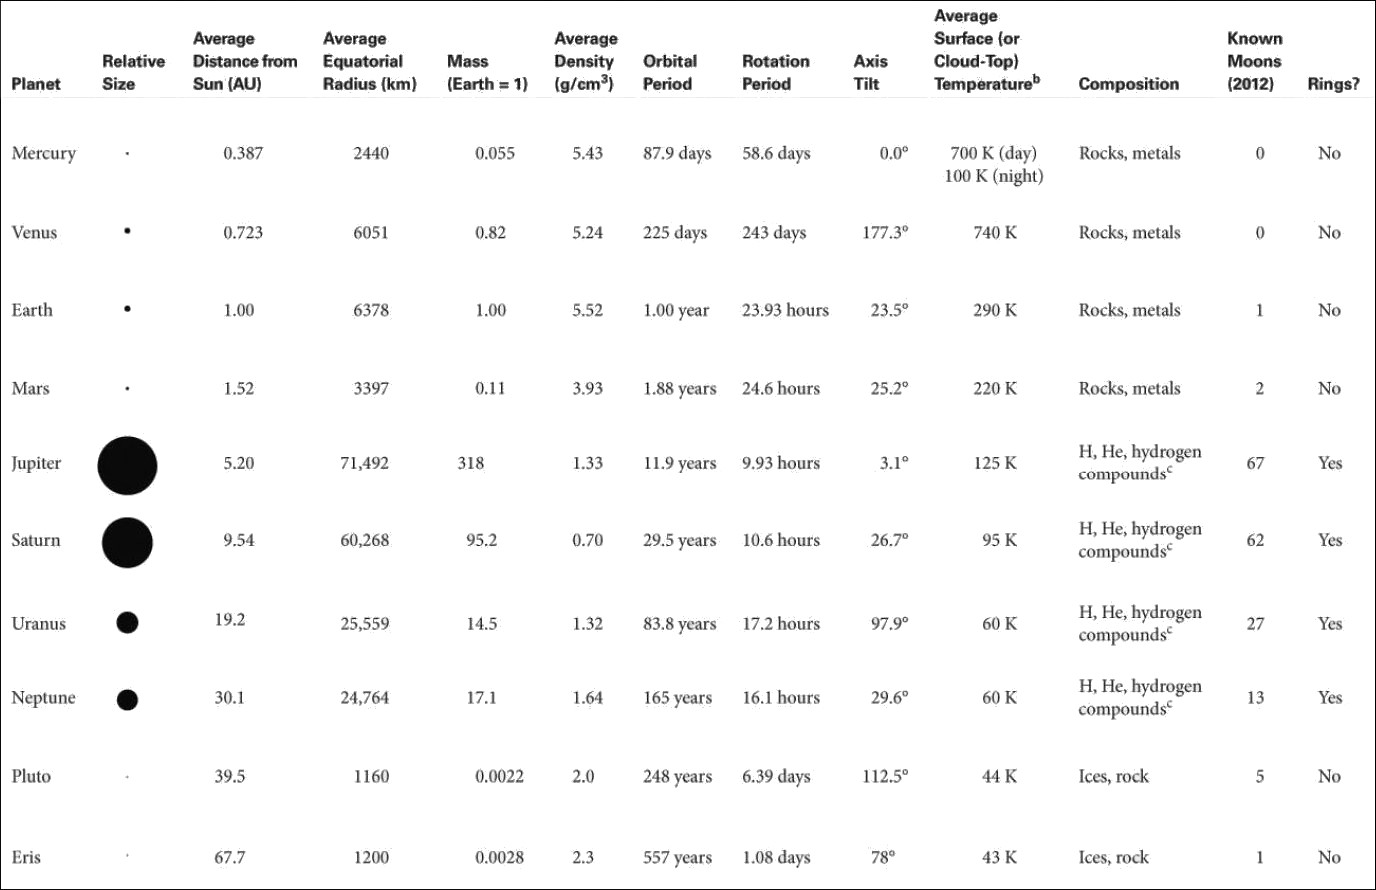
\includegraphics[angle=90,scale=0.5]{planetData}

\subsubsection{Spacecraft Exploration}
\textbf{Flyby}: flys past a planet (usually a slingshot type path), cheapest but gathers less data

\textbf{Orbiters}: go into orbit around object, more time to gather data

\textbf{Probes and Landers}: land on surface, most expensive

\textbf{Combination}: an orbiter drops a lander and continues its orbit
